\chapter{从波的叠加到一个反问题}
\section{探测器测到了什么}
设入射、出射波矢分别为 $k_0,k_1$，采用不含 $2\pi$ 的约定，$\|k_0\|=\|k_1\|=1/\lambda$。位于 $r$ 的一个电子相对于原点产生相位差 $2\pi(k_1-k_0)\cdot r$。晶胞电子密度为 $\rho(r)$ 时，散射振幅是各位置的复振幅之和：
\begin{equation}
 F(q)=\int_{\text{cell}}\rho(r)\exp(2\pi\iu q\cdot r)\,\dif r,
 \qquad q=k_1-k_0 .
\end{equation}
晶格的周期重复使这些波只在倒易晶格附近相长叠加。令 $q=Bh$、$r=Ax$，因为 $B^{\mathsf T}A=I$，有 $q\cdot r=h\cdot x$。这就是 Miller 指数和分数坐标能直接出现在相位里的原因。

普通 X 射线探测器统计到达的光子或由它们形成的电荷，没有记录波的相位。理想衍射强度与 $|F_h|^2$ 成正比，但原始像素还包含背景、有限峰宽、几何因子、吸收和探测器噪声。软件的基本任务因此是反推一组能够产生这些像素的物理参数。

\section{原子模型与温度因子}
若电子密度是各原子电子云的叠加，原子发生均值为零、协方差为 $U_j$ 的高斯位移，则位移的特征函数给出
\begin{equation}
 \E\{\exp(2\pi\iu q\cdot u_j)\}=\exp(-2\pi^2q^{\mathsf T}U_jq).
\end{equation}
定义 $s=\sin\theta/\lambda=\|q\|/2$，其中 $2\theta$ 是散射角；$s$ 与 $q$ 的单位均为倒数长度。因此结构因子可以写为
\begin{equation}\label{eq:structure-factor}
 F_h(\theta)=\sum_j\sum_{o\in G/H_j}o_j
 \left[f^0_j(s)+f'_j+\iu f''_j\right]
 \exp\!\left[-2\pi^2q^{\mathsf T}U_{jo}q+2\pi\iu h^{\mathsf T}x_{jo}\right].
\end{equation}
$G$ 是空间群，$H_j$ 是保持位置 $j$ 不变的稳定子群。商 $G/H_j$ 的作用是只对不同的物理位置求和。一个位于反演中心、完整占据的原子，占有率仍是 1；不能因为若干对称操作得到同一位置，就把它重复计数或任意修改占有率。

当 $U_j=u_jI$ 时，指数退化为 $-8\pi^2u_js^2$。非球形热运动则必须保留张量。旋转对称操作也要旋转张量；只旋转坐标、保持各向异性张量不动，会在高角反射中产生系统误差。

本包用 Gemmi 提供的 IT92 中性原子散射系数和空间群表，自行计算式\eqref{eq:structure-factor}及其导数。$f'$、$f''$ 是显式输入，不把波长依赖或反常散射自动猜进去。这里采用运动学 X 射线模型；多重散射强烈的电子衍射需要额外的前向模型。

\section{相干叠加与孪晶的非相干叠加}
同一有序晶胞内的原子先加振幅，再取平方；通常的宏观孪晶畴之间采用非相干强度混合：
\begin{equation}\label{eq:twin-intensity}
 \mu_h=k\sum_{d=1}^{D}\alpha_d\,|F_{T_dh}(\theta)|^2,
 \quad \alpha_d\ge0,\quad\sum_d\alpha_d=1.
\end{equation}
两种求和顺序不能互换。$|F_1+F_2|^2$ 含有干涉交叉项，通常不能用于描述独立孪晶畴的完全重叠。对于非面网孪晶，某个探测器区域可能只重叠一部分反射；这时每个分量有自己的索引和像素轮廓，应回到更一般的模型
\begin{equation}\label{eq:pixel-forward}
 \mu_i=b_i+\sum_j P_{ij}(\eta)c_j(\eta)\alpha_{d(j)}k|F_{h_j}(\theta)|^2 .
\end{equation}
$\eta$ 包含仪器几何与轮廓参数，$c_j$ 包含已经明确的相对标度与校正因子。式\eqref{eq:pixel-forward}将像素处理与结构精修接成了同一个问题。

\section{信息在哪一步丢失}
把像素压缩成强度表并不一定丢失有用信息。关键在于保留的数据是否足以对所有候选结构计算同一个似然。固定方差的线性高斯模型存在精确的有限维压缩；一般泊松像素模型则不能随意压成一个强度和一个标准差。

相位丢失是另一件事。设 $F_h=|F_h|e^{\iu\phi_h}$，在不改变 $|F_h|$ 的情况下改变相位，可以得到完全不同的电子密度。图\ref{fig:phase-basic}展示了这一点。相位求解必须引入原子性、密度约束、对称性或化学组成等额外信息。
\begin{figure}[!htbp]
\centering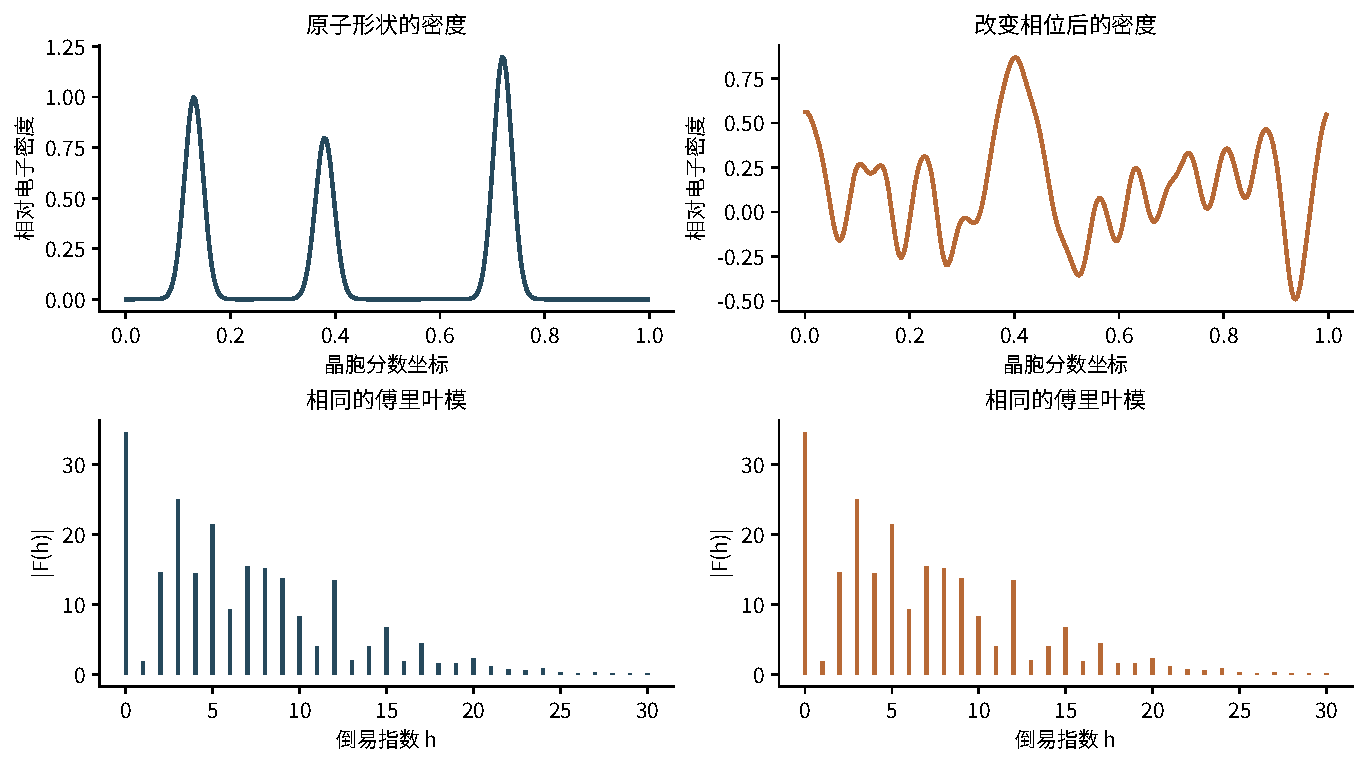
\includegraphics[width=\textwidth]{figures/01_phase_problem.pdf}
\caption{一维教学模型。两组傅里叶系数具有相同的模，但相位不同，得到的实空间密度明显不同。上方的原子峰与下方的相位扰动密度都由随附绘图脚本直接计算；它们不是实验数据。}\label{fig:phase-basic}
\end{figure}

\begin{principle}
从像素到结构的每一步都应回答两个问题：前向模型是什么？哪些未知量能由当前数据区分？速度优化只有在不改变这两个问题的含义时，才是可靠的优化。
\end{principle}
